%!TEX root = ../../main.tex


\begin{figure}[p]
\centering
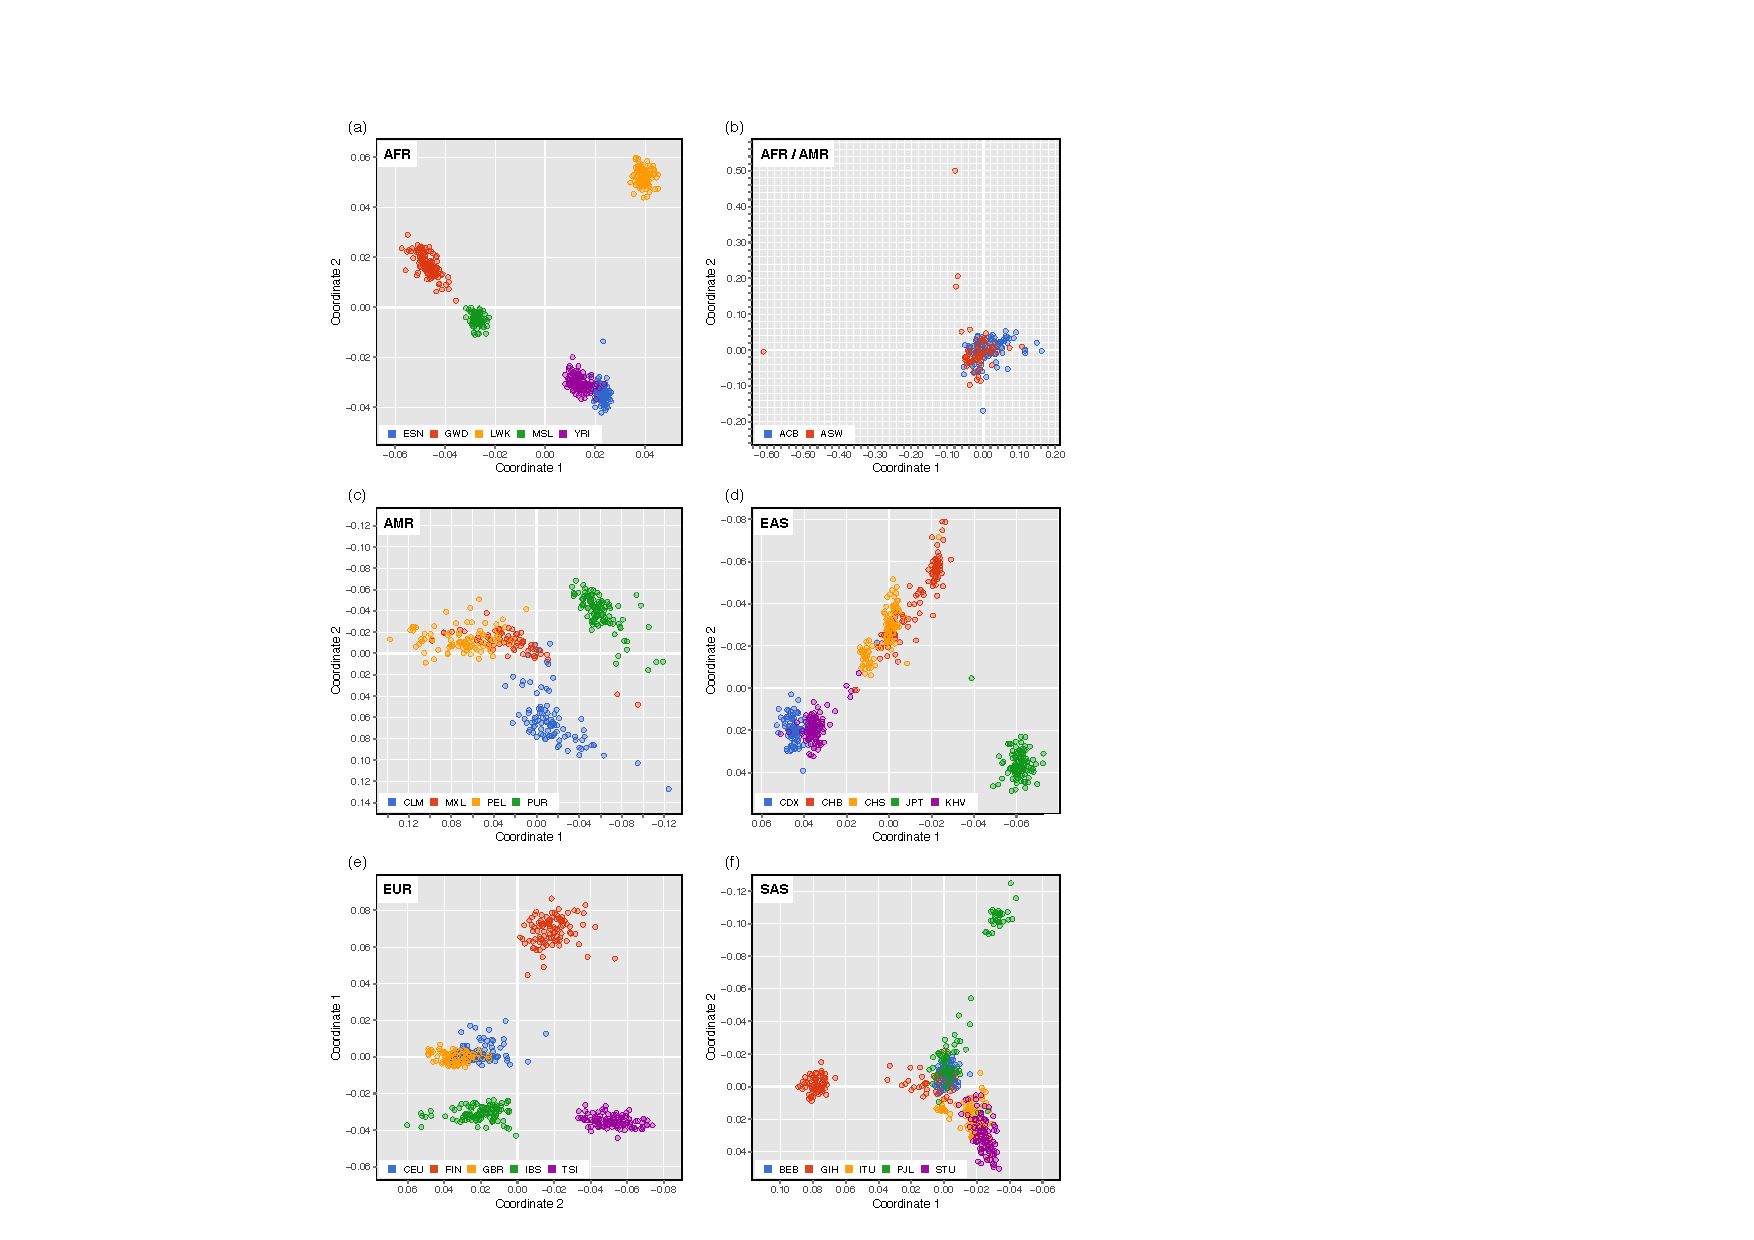
\includegraphics[width=0.9\textwidth]{./img/ch3/pcoa_1kg}
\Caption{Principal coordinates analysis of pairwise shared rare variants}
{...

Axis orientation in each panel was chosen to better reflect the cardinal directions on a geographic map; \ie the top, bottom, left and right sides of each panel roughly correspond to North, South, West, and East, respectively.
Note that the colours used do not adhere to the colour-scheme defined in the \glsentrylong{1kg}; instead, arbitrary colours were chosen to better distinguish population groups.

...}
{fig:pcoa_1kg}
% \vspace{-5pt}
% \hrulefill%
\end{figure}
